\documentclass[11pt]{article}
\usepackage[utf8]{inputenc}
\usepackage{lipsum}    % for placeholder text (remove if not needed)
\usepackage{graphicx}  % if you need to include images
\usepackage{amsmath}   % if you need math
\usepackage{amssymb}   % if you need more math symbols
\usepackage{booktabs}  % for nicer tables
\usepackage{csvsimple} % For displaying CSV files
\usepackage{booktabs} % For better table formatting


\title{Machine Learning Based Algorithmic Trading}
\author{Md Kauser Ahmmed}
\date{\today}

\begin{document}

\maketitle

% \section{Introduction}
% This report outlines the steps and requirements for the class project, titled \textit{Machine Learning Based Algorithmic Trading}. The main tasks include data collection, observation exclusions, feature engineering, model building, and back-testing a trading strategy. Below is a structured summary of each stage.

\section{Data Collection}
We collect historical data of eleven assets (e.g., stocks, ETFs). The following table shows the assets and associated data parameters:

\begin{table}[ht]
    \centering
    \begin{tabular}{|l|l|l|l|}
        \hline
        \textbf{Asset Name} & \textbf{Time Period} & \textbf{Frequency} & \textbf{Source of Data} \\ \hline
        TSLA                & 2 years              & 1 min              & Alpha Vantage           \\ \hline
        AAPL                & Jan 2023 -- Dec 2024 &                   &                         \\ \hline
        NVDA                &                      &                   &                         \\ \hline
        AMD                 &                      &                   &                         \\ \hline
        AMZN                &                      &                   &                         \\ \hline
        MSFT                &                      &                   &                         \\ \hline
        NFLX                &                      &                   &                         \\ \hline
        XOM                 &                      &                   &                         \\ \hline
        META                &                      &                   &                         \\ \hline
        NKE                 &                      &                   &                         \\ \hline
        S\&P 500            &                      &                   &                         \\ \hline
    \end{tabular}
    \caption{Asset Data Parameters}
    \label{tab:asset_data}
\end{table}

\begin{table}[h!]
    \centering
    \begin{tabular}{|l|l|p{5cm}|} % Adjusted width for better readability
        \hline
        \textbf{Cluster (Sector)} & \textbf{Assets} & \textbf{Rationale} \\ \hline
        Technology & AAPL, AMD, MSFT, NVDA & Companies in semiconductors, consumer electronics, and software. \\ \hline
        Communication Services & META, NFLX & Focus on digital media, social networking, and streaming services. \\ \hline
        Consumer Discretionary & AMZN, TSLA, NKE & Industries tied to consumer spending: retail, automotive, and apparel. \\ \hline
        Energy & XOM & Major oil \& gas company with distinct sector dynamics. \\ \hline
        Diversified ETF & SPY & Tracks the S\&P 500, representing the overall market. \\ \hline
    \end{tabular}
    \caption{Clusters of Assets Based on Sectors}
    \label{tab:clusters}
\end{table}

% \begin{itemize} 
%     \item \textbf{Data source:} Alpha Vantage API is used to retrieve the necessary price (open, high, low, close) and volume data.
%     \item \textbf{Time horizon:} 1 minute interval data of 2 years (January 2023 - December 2024).
% \end{itemize}

\newpage

\section{Observation Exclusions}
Only one exclusion principle is applied upto now. Work in progress for additional exclusion logics.

\begin{table}[h!]
    \centering
    \caption{Summary of Observation Exclusion Techniques}
    \label{tab:observation_exclusion_technique}
    \begin{tabular}{|l|p{8cm}|}
        \hline
        \textbf{Step} & \textbf{Description} \\ \hline
        Time-Based Exclusion & Rows with timestamps outside the range \texttt{[10, 15]} (10 AM to 3 PM) are excluded. \\ \hline
    \end{tabular}
\end{table}

\begin{figure}[ht]
    \centering
    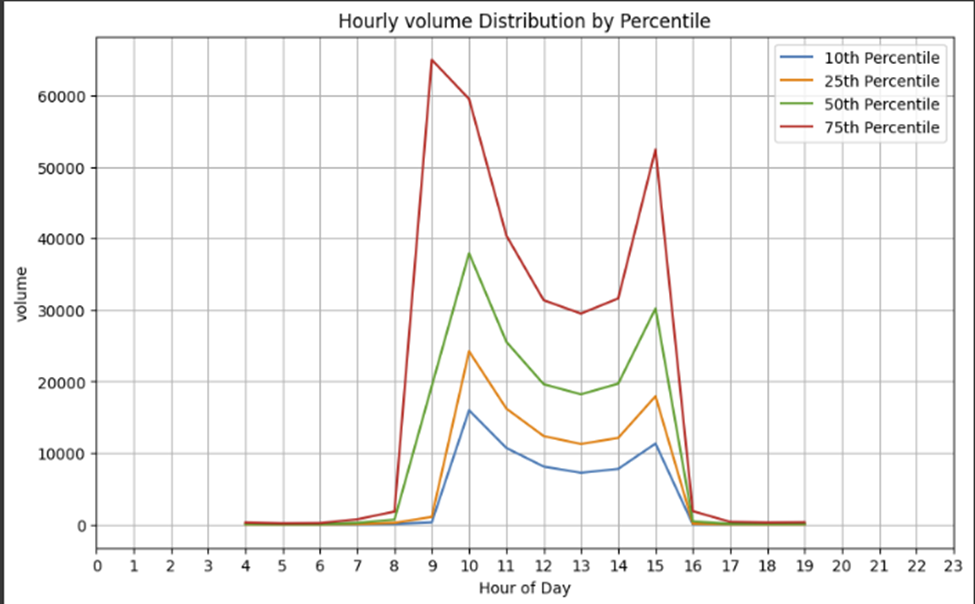
\includegraphics[width=0.8\textwidth]{exclusion_hour_of_day_1.png}
    \caption{Exclusion Criteria Based on Hour of Day. Data outside the desired trading hours are excluded. ($<10$ AM or $>3$ PM)}
    \label{fig:exclusion_hour}
\end{figure}

% \begin{figure}[ht]
%     \centering
%     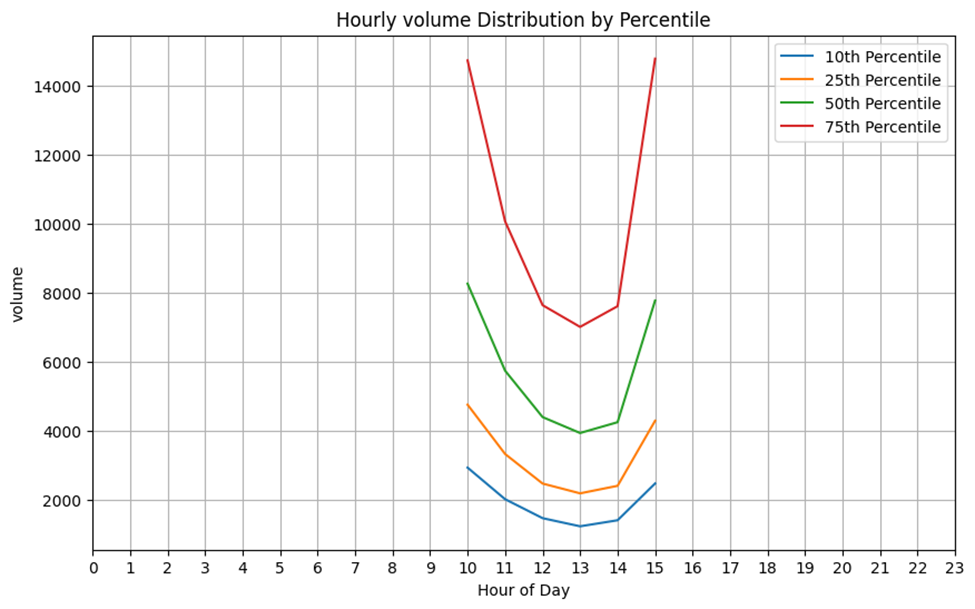
\includegraphics[width=0.8\textwidth]{exclusion_hour_of_day_2.png}
%     \caption{After the observation is excluded Based on Hour of Day.}
%     \label{fig:after_exclusion_hour}
% \end{figure}

\newpage
% \section{Data Processing}
% \begin{itemize}
%     \item \textbf{Cleaning features:} Handle missing values (impute or remove) and ensure that any extreme outliers are either capped or removed based on your exclusion rule.
%     \item \textbf{Resampling or alignment:} If data come at different frequencies or have different time zones, ensure proper alignment before feature generation.
% \end{itemize}

\section{Feature Generation}

\subsection*{Feature Types}
The features are categorized into two types:
\begin{itemize}
    \item \textbf{Binary Features}: These are indicator variables (e.g., flags for crossovers, thresholds) that take on values of 0 or 1.
    \item \textbf{Continuous Features}: These are numerical variables (e.g., moving averages, volatility measures, RSI) that capture quantitative aspects of the data.
\end{itemize}

\begin{table}[h!]
    \centering
    \begin{tabular}{|l|l|l|}
    \hline
    \textbf{Feature Category} & \textbf{Period} & \textbf{Feature Type} \\ \hline
    Binary\_SMA\_Crossover & Short$|$Long: 120$|$240, 240$|$480, 
                            ...% 480$|$960, 960$|$1920, 1920$|$3840 
                            & binary \\ \hline
    Price\_Above\_VWAP & 120, 240, 480, 960, 1920 & binary \\ \hline
    MACD\_Bullish & fast$|$slow$|$signal: 120$|$240$|$90, 240$|$480$|$120
                ...% , 480$|$960$|$240, 960$|$1920$|$480, 1920$|$3840$|$960 
                & binary \\ \hline
    RSI & 120, 240, 480, 960, 1920 & continuous \\ \hline
    RSI\_Threshold & lower$|$upper: 15$|$85, 20$|$80, 25$|$75, 30$|$70, 35$|$65 & binary \\ \hline
    BB\_Breakout & 120, 240, 480, 960, 1920 & binary \\ \hline
    SMA\_cont & 120, 240, 480, 960, 1920 & continuous \\ \hline
    ATR & 120, 240, 480, 960, 1920 & continuous \\ \hline
    Momentum & 120, 240, 480, 960, 1920 & continuous \\ \hline
    Average\_Return & 120, 240, 480, 960, 1920 & continuous \\ \hline
    Rate\_Close\_Greater\_Open & 120, 240, 480, 960, 1920 & continuous \\ \hline
    Downside\_Deviation & 120, 240, 480, 960, 1920 & continuous \\ \hline
    Sortino\_Ratio & 120, 240, 480, 960, 1920 & continuous \\ \hline
    Max\_Close & 120, 240, 480, 960, 1920 & continuous \\ \hline
    Min\_Close & 120, 240, 480, 960, 1920 & continuous \\ \hline
    Open &  & continuous \\ \hline
    Close &  & continuous \\ \hline
    High &  & continuous \\ \hline
    Low &  & continuous \\ \hline
    Volume &  & continuous \\ \hline
    Total Number of Features & 103 &  \\ \hline
    \end{tabular}
    \caption{Feature Categories with Periods and Feature Types}
    \label{tab:features}
\end{table}
\newpage

\section{Train--Test Split}
\begin{itemize}
    \item Train: 70\%
    \item Test1: 15\%
    \item Test2: 15\%
\end{itemize}
\newpage
% \section{Data Processing}
% \begin{itemize}
%     \item \textbf{At least 2 test samples:} Partition your historical data into multiple segments (e.g., a train set and two test sets). 
%     \item \textbf{Walk-forward approach (optional):} Consider a time-series cross-validation method for more robust evaluation.
% \end{itemize}

\section{Feature Reduction}
Use XGBoost to get feature importance. First used a default xgboost model, filter feature importance with a threshold of 0.0145. Then filter a XGBoost model with parameter and same threshold. Then from the combined feature importance, get the significant features in both of the filtered important features. Rest of the features are removed.
\begin{figure}[ht]
    \centering
    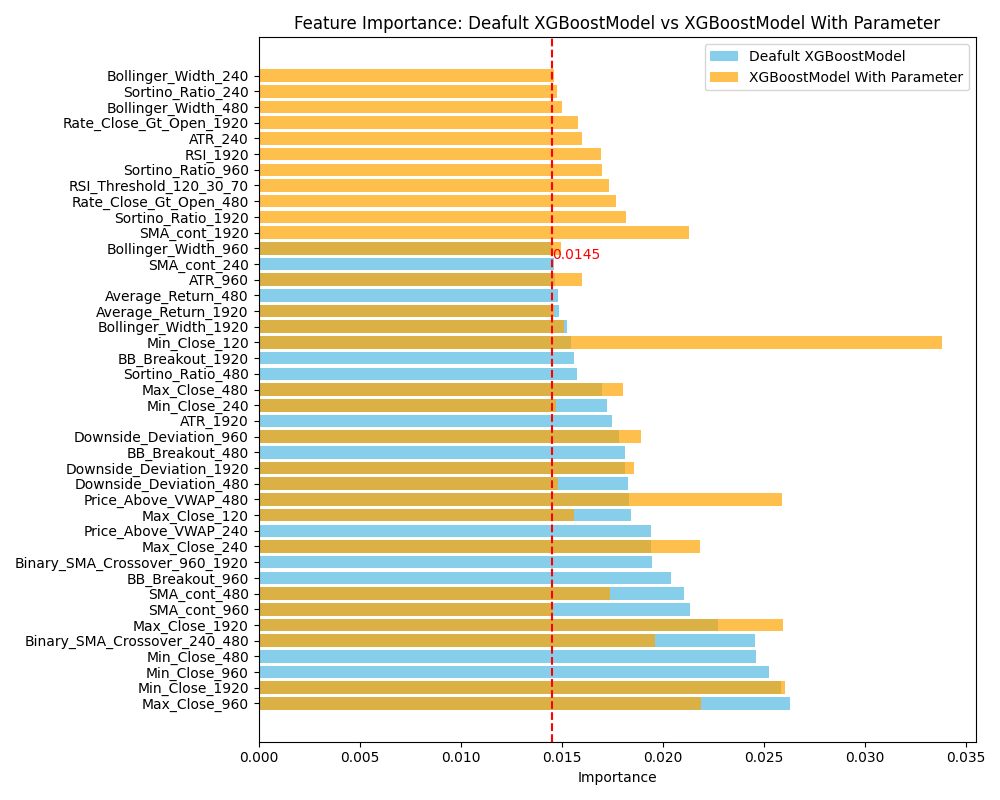
\includegraphics[width=0.8\textwidth]{AMZN/feature_importance_comparison.png}
    \caption{Feature Importance using XGBOOST Model}
    \label{fig:feature_importance}
\end{figure}
\newpage



\section{Grid Search}
\begin{figure}[ht]
    \centering
    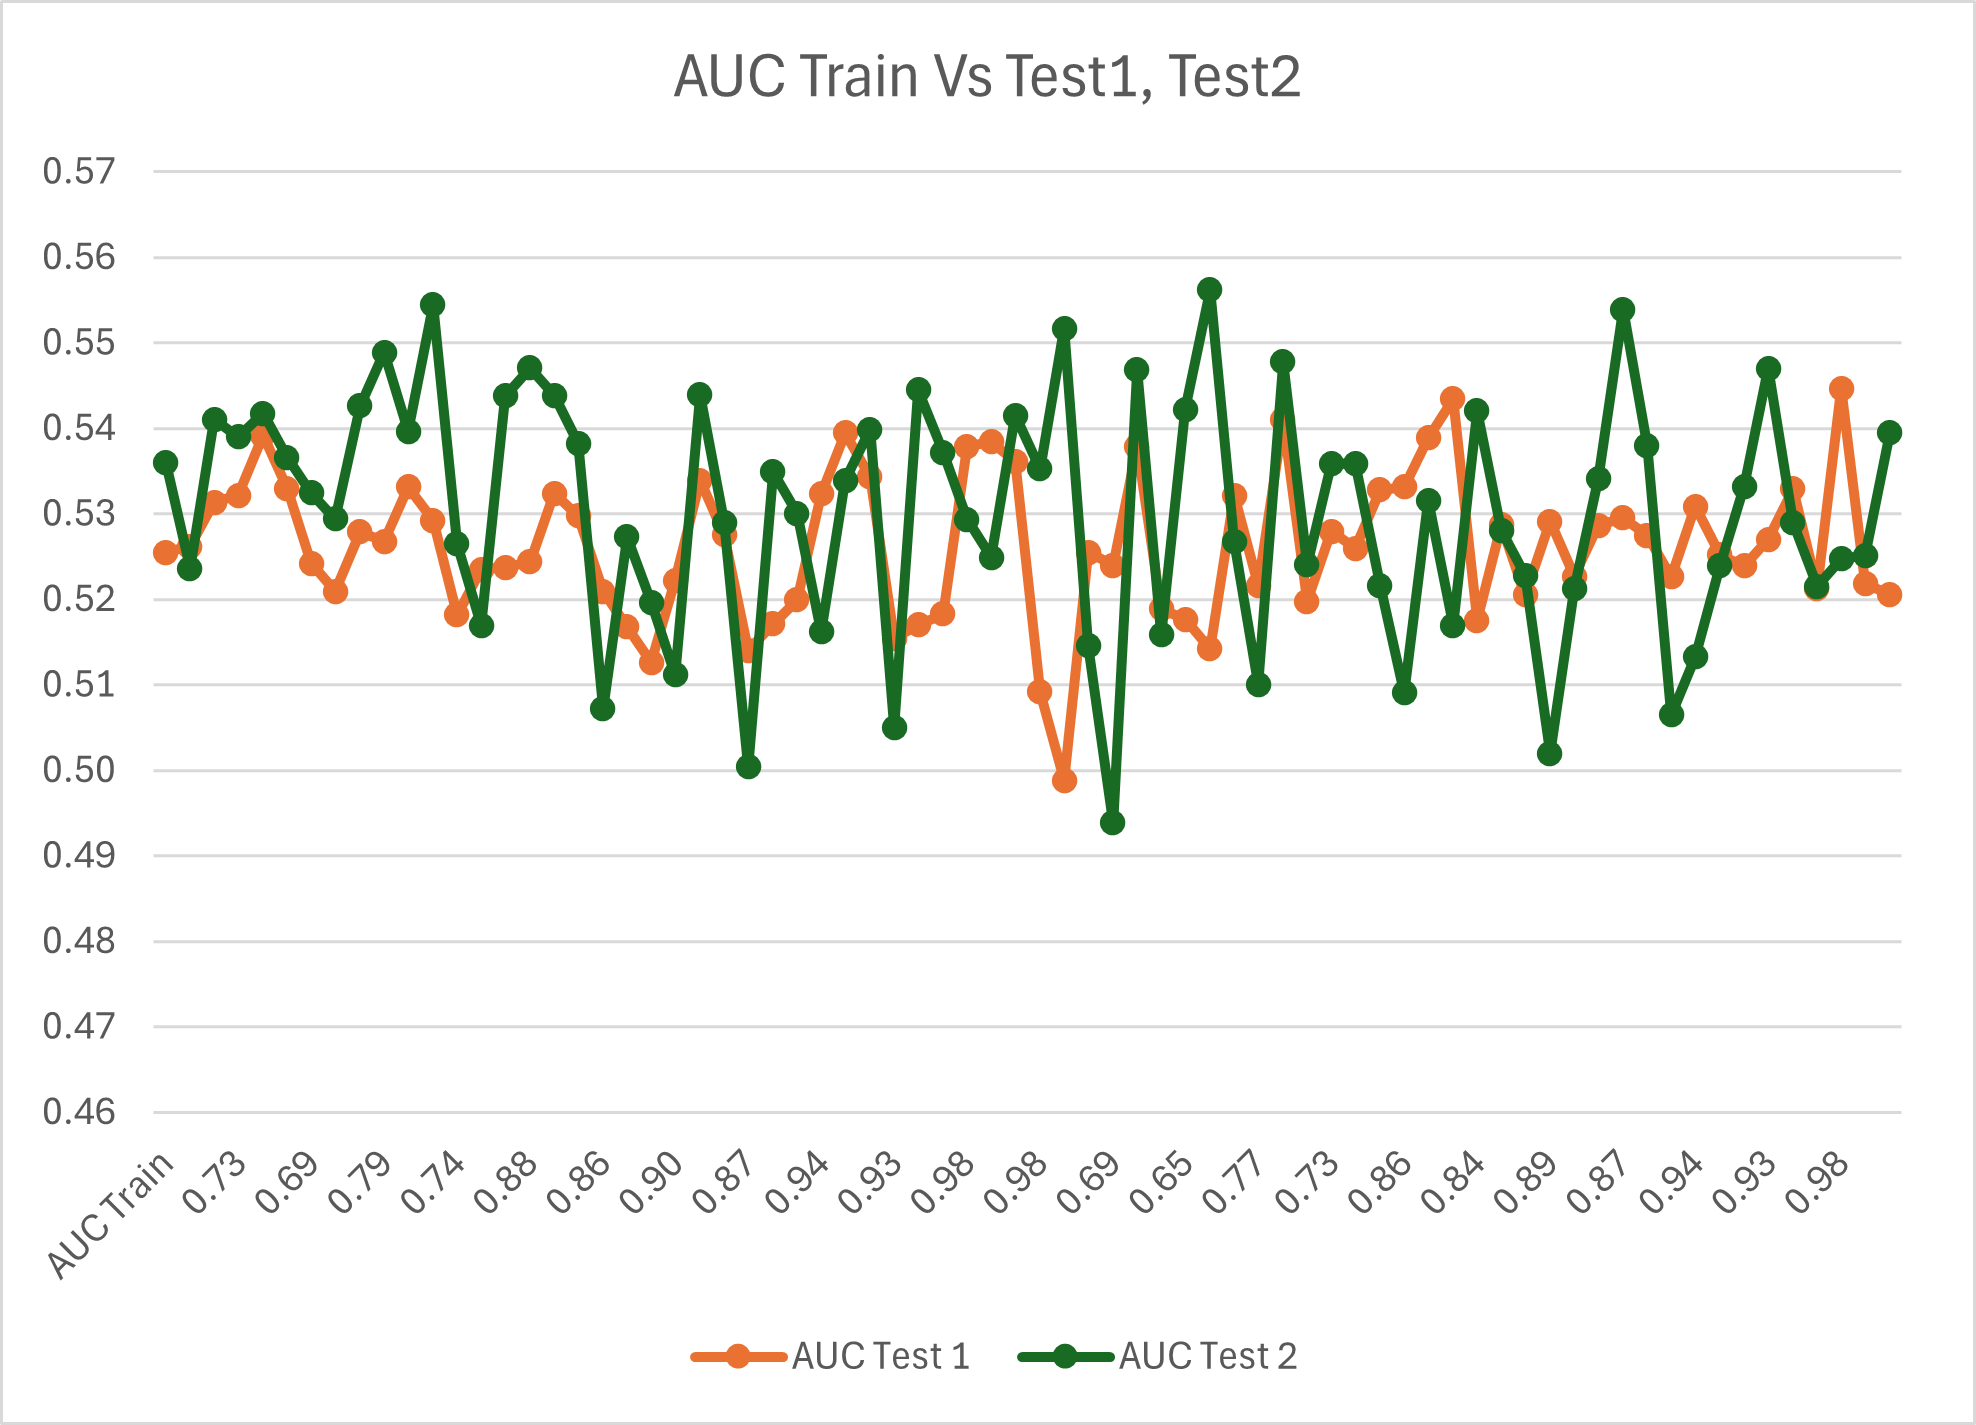
\includegraphics[width=0.8\textwidth]{AMZN_AUC_TRAIN_VS_TEST1_TEST2.png}
    \caption{Grid Search Results XGBOOST Model}
    \label{fig:grid_search_results}
\end{figure}
\newpage

\section{Shap Analysis}
\begin{figure}[ht]
    \centering
    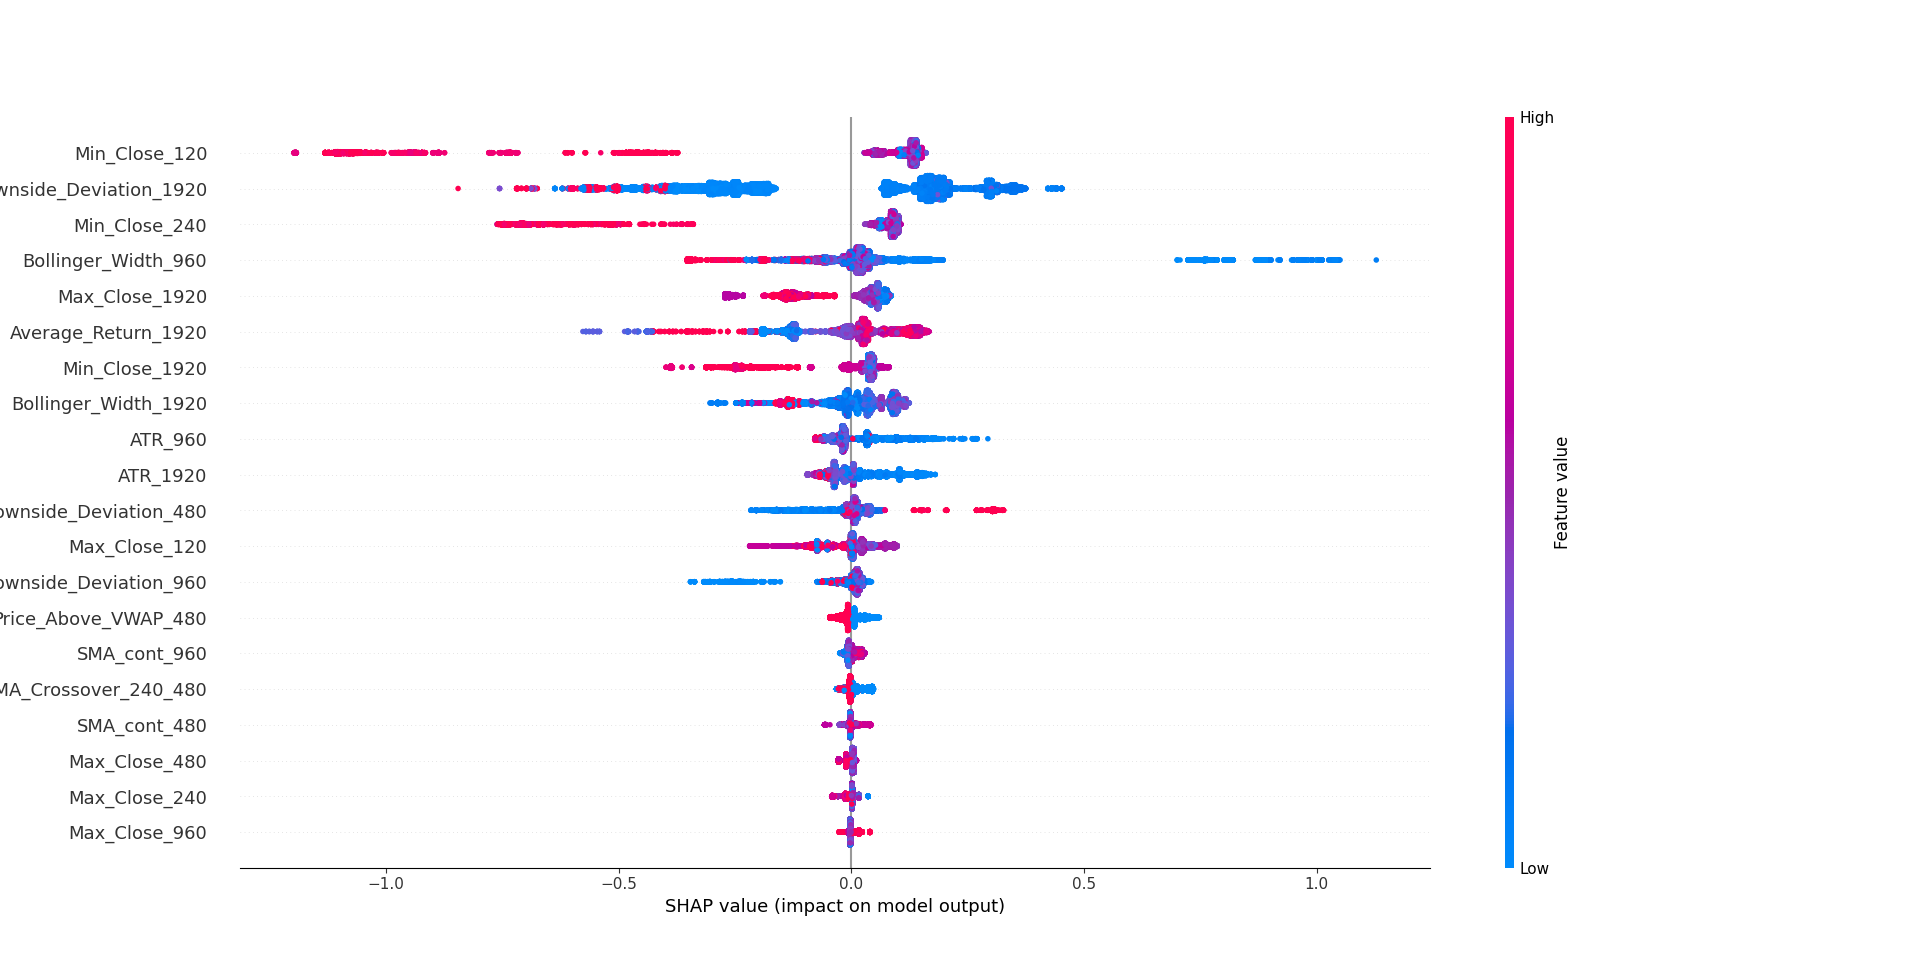
\includegraphics[width=1.2\textwidth]{AMZN/shap_analysis_beeswarm.png}
    \caption{Shap Analysis: beeswarm for Test1 dataset}
    \label{fig:shap_analysis_beeswarm_1}
\end{figure}

\begin{figure}[ht]
    \centering
    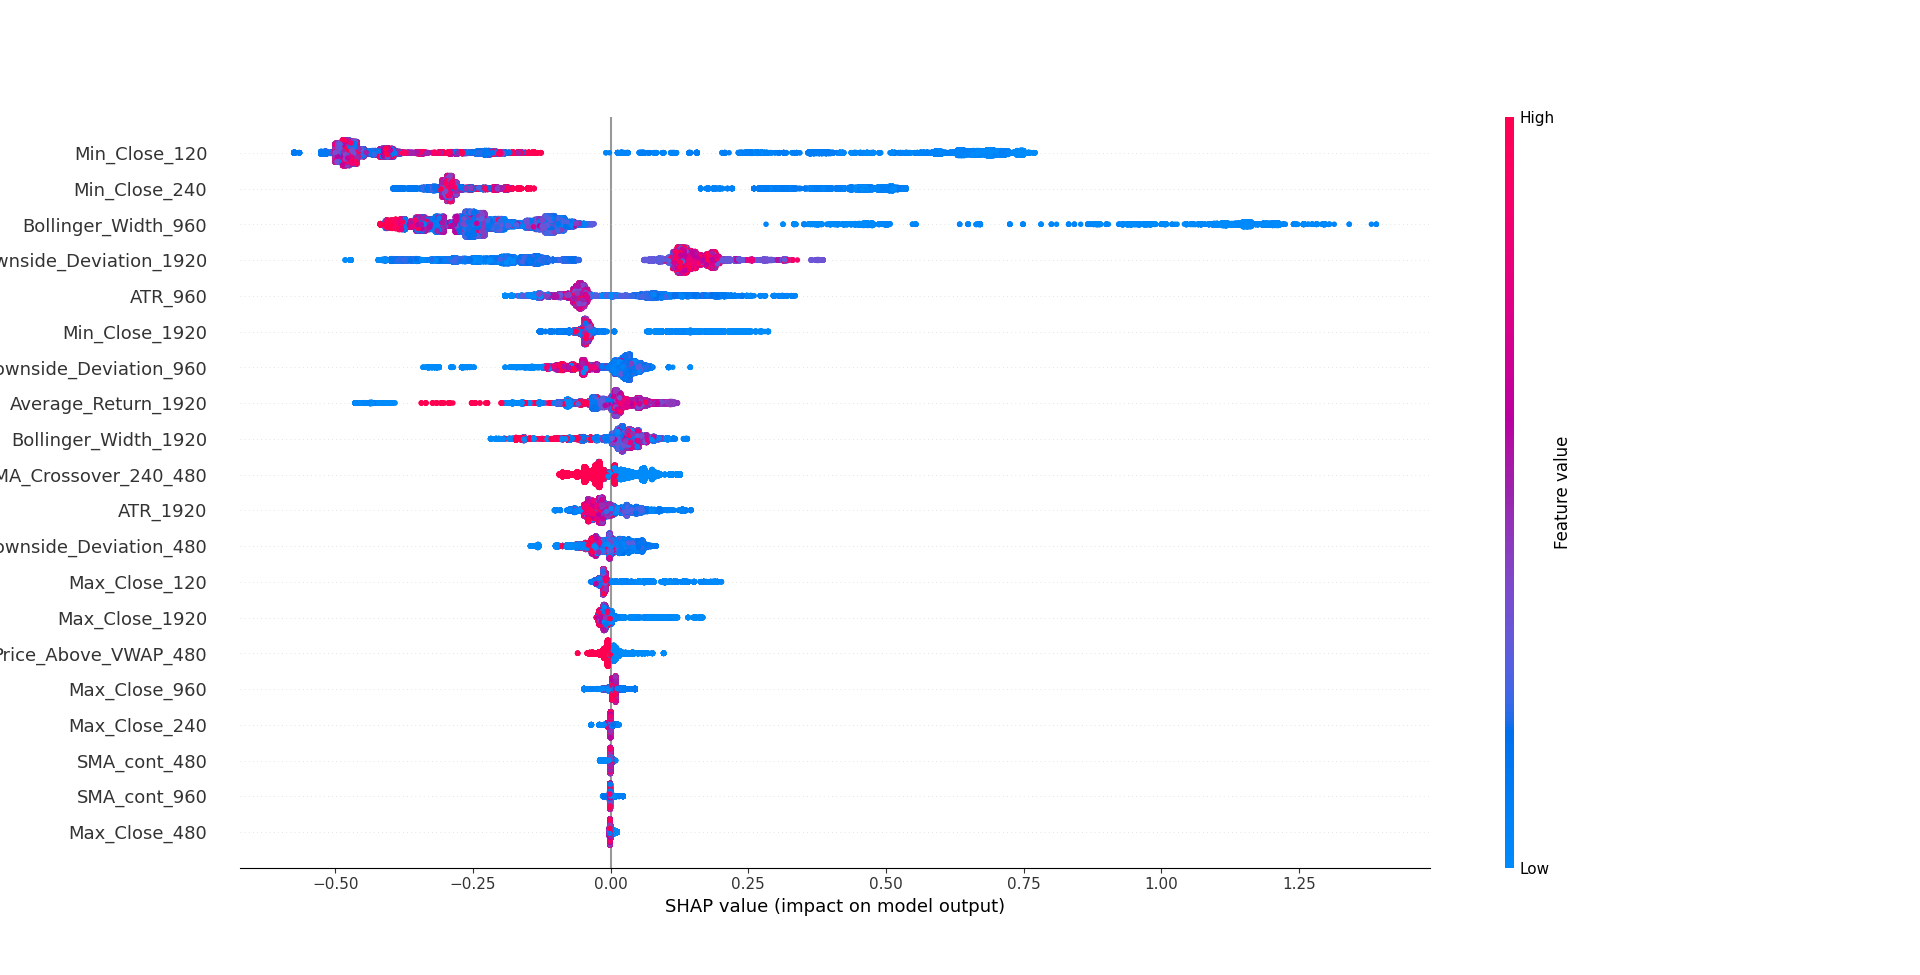
\includegraphics[width=1.2\textwidth]{AMZN/shap_analysis_beeswarm_test_2.png}
    \caption{Shap Analysis: beeswarm for Test2 dataset}
    \label{fig:shap_analysis_beeswarm_2}
\end{figure}

\begin{figure}[ht]
    \centering
    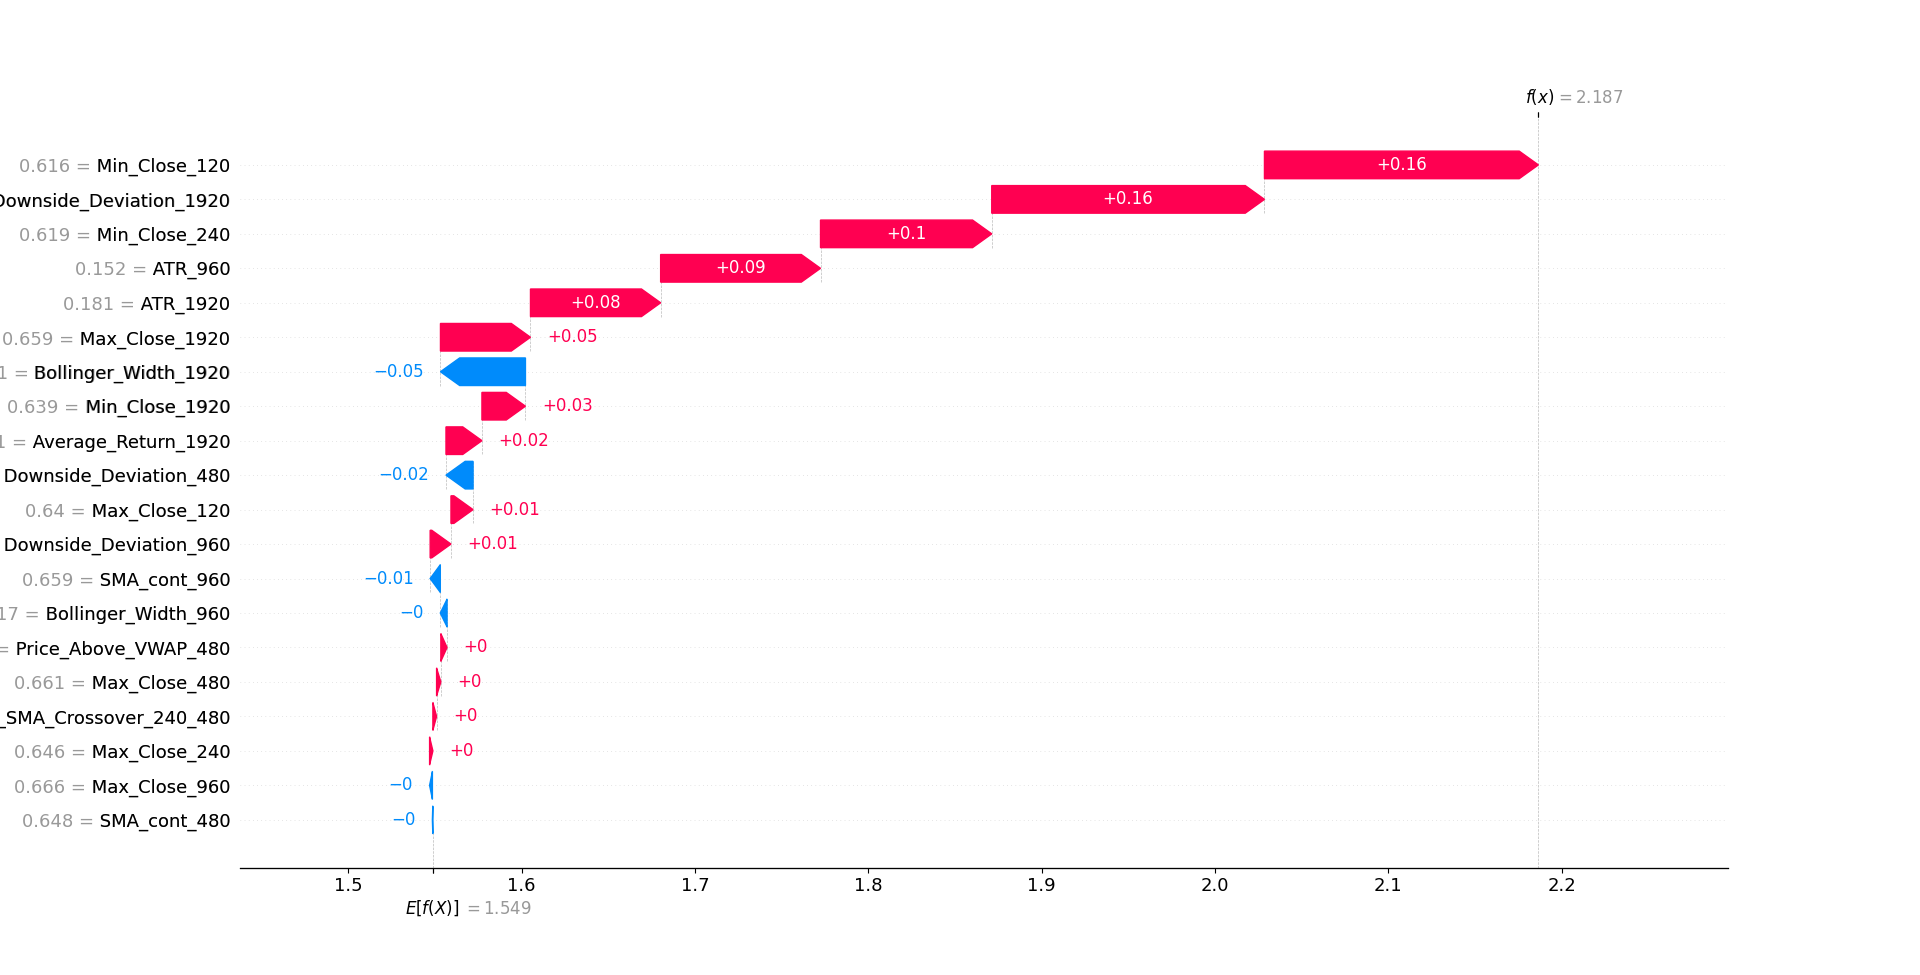
\includegraphics[width=1.2\textwidth]{AMZN/shap_analysis_waterfall_test_1_observation_1000.png}
    \caption{Shap Analysis: Waterfall for obervation number 1000 on TEST1 dataset}
    \label{fig:shap_analysis_waterfall_1}
\end{figure}

\newpage



% \section{Feature Selection \& Model Building}
% \begin{itemize}
%     \item \textbf{Model pipeline:} Use a machine learning pipeline that includes:
%     \begin{itemize}
%         \item Data scaling or normalization (if needed).
%         \item Feature selection (optional or integrated into the model).
%         \item An estimator (e.g., XGBoost, Random Forest, or a simpler model).
%     \end{itemize}
%     \item \textbf{Cross-validation:} Evaluate model performance using cross-validation (e.g., $k$-fold or walk-forward for time series).
%     \item \textbf{Hyperparameter tuning:} Employ a grid search (or similar) to find the best model parameters.
%     \item \textbf{Threshold/Strategy logic:} If using a threshold for classification or a target variable for regression, define how signals are derived (e.g., predicted probability $>0.6$ triggers a trade).
% \end{itemize}



\section{Strategy Definition}
The goal is to identify the optimal trading strategy by selecting the best threshold in conjunction with a defined trade setup. Note that strategy performance depends on both the predictive model (and its threshold) and the trade setup parameters. The key components of our methodology are as follows:

\subsection*{Trade Setup Definition}
\begin{itemize}
    \item \textbf{Holding Period:} The maximum number of periods a trade is held before closing.
    \item \textbf{Take Profit:} The profit target (e.g., 0.5\% or 1\%) that triggers an early exit.
    \item \textbf{Stop Loss:} The loss limit (e.g., -0.5\% or -1\%) at which the trade is terminated to control risk.
\end{itemize}

\subsection*{Strategy Simulation}
\begin{itemize}
    \item A trade is initiated when the predicted signal (derived from the model) meets or exceeds a specified threshold.
    \item Once entered, the trade is held for up to the defined holding period.
    \item The trade is exited early if:
    \begin{itemize}
         \item The return reaches or exceeds the \textbf{Take Profit} level, or
         \item The return falls below the \textbf{Stop Loss} level.
    \end{itemize}
    \item If neither condition is met, the trade is closed at the end of the holding period.
\end{itemize}

\subsection*{Performance Metrics}
For each strategy configuration, the following metrics are computed:
\begin{itemize}
    \item \textbf{Number of Trades:} Total trades executed.
    \item \textbf{Win Rate:} Proportion of trades with positive returns.
    \item \textbf{Total Return:} Cumulative return over all trades.
    \item \textbf{Sharpe Ratio:} Ratio of the average trade return to the standard deviation of returns, representing risk-adjusted performance.
\end{itemize}

\subsection*{Grid Search and Back-testing}
\begin{itemize}
    \item A grid search is conducted over various combinations of the trade setup parameters and threshold values.
    \textbf{Holding Periods:} 60, 120, 240 periods.
    \textbf{Take Profit:} 0.005, 0.01.
    \textbf{Stop Loss:} -0.005, -0.01.
    \textbf{Thresholds:} 0.5, 0.6, 0.7, 0.8, 0.9.
    
    \item For each parameter combination, the strategy is simulated using the development sample (Test + Train), and the performance metrics are recorded.
    \item The results are compiled into a table for further analysis.
\end{itemize}

\subsection*{Best Strategy Selection}
\begin{itemize}
    \item The best configuration is chosen based on the highest Sharpe.
    \item This configuration is then adopted for further model deployment and strategy implementation.
\end{itemize}


\section{Back-Testing \& Results}
\begin{figure}[ht]
    \centering
    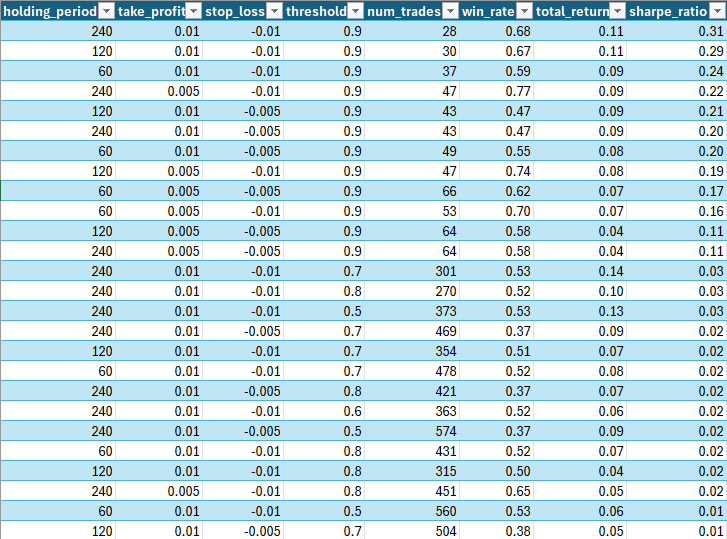
\includegraphics[width=1.2\textwidth]{AMZN/strategy _result_for_test_1.png}
    \caption{Backtesting: Performance of strategy on Test1 dataset}
    \label{fig:backtesting_strategy_test1}
\end{figure}

% \begin{itemize}
%     \item \textbf{Implement the strategy:} Simulate trades over your test period(s).
%     \item \textbf{Performance metrics:} 
%     \begin{itemize}
%         \item Sharpe ratio or Sortino ratio (risk-adjusted returns).
%         \item Win rate, total return, maximum drawdown, etc.
%     \end{itemize}
%     \item \textbf{Plots:} Provide time-series plots of:
%     \begin{itemize}
%         \item Asset price and trades marked (entry/exit).
%         \item Equity curve (portfolio value over time).
%         \item Feature values (optional).
%     \end{itemize}
% \end{itemize}

% \section{Conclusion}
% Summarize your findings, including:
% \begin{itemize}
%     \item Which features appeared most important based on the model.
%     \item Which hyperparameters or thresholds yielded the best performance.
%     \item Potential improvements (e.g., more data, different models, more advanced feature engineering).
% \end{itemize}

% \section{References}
% \begin{itemize}
%     \item Data source (e.g., Alpha Vantage, Yahoo Finance).
%     \item Any libraries or packages used (e.g., scikit-learn, xgboost, pandas).
% \end{itemize}

\end{document}
